\documentclass[11pt]{article}

% Change "review" to "final" to generate the final (sometimes called camera-ready) version.
% Change to "preprint" to generate a non-anonymous version with page numbers.
\usepackage[final]{acl}

% Standard package includes
\usepackage{times}
\usepackage{latexsym}
\usepackage[flushleft]{threeparttable} % http://ctan.org/pkg/threeparttable
\usepackage{booktabs,caption}

% For proper rendering and hyphenation of words containing Latin characters (including in bib files)
\usepackage[T1]{fontenc}
% For Vietnamese characters
% \usepackage[T5]{fontenc}
% See https://www.latex-project.org/help/documentation/encguide.pdf for other character sets

% This assumes your files are encoded as UTF8
\usepackage[utf8]{inputenc}

% This is not strictly necessary, and may be commented out,
% but it will improve the layout of the manuscript,
% and will typically save some space.
\usepackage{microtype}

% This is also not strictly necessary, and may be commented out.
% However, it will improve the aesthetics of text in
% the typewriter font.
\usepackage{inconsolata}

%Including images in your LaTeX document requires adding
%additional package(s)
\usepackage{graphicx}

% If the title and author information does not fit in the area allocated, uncomment the following
%
%\setlength\titlebox{<dim>}
%
% and set <dim> to something 5cm or larger.

\title{CAS 732: Replication Project Progress Report}

% Author information can be set in various styles:
% For several authors from the same institution:
% \author{Author 1 \and ... \and Author n \\
%         Address line \\ ... \\ Address line}
% if the names do not fit well on one line use
%         Author 1 \\ {\bf Author 2} \\ ... \\ {\bf Author n} \\
% For authors from different institutions:
% \author{Author 1 \\ Address line \\  ... \\ Address line
%         \And  ... \And
%         Author n \\ Address line \\ ... \\ Address line}
% To start a separate ``row'' of authors use \AND, as in
% \author{Author 1 \\ Address line \\  ... \\ Address line
%         \AND
%         Author 2 \\ Address line \\ ... \\ Address line \And
%         Author 3 \\ Address line \\ ... \\ Address line}

\author{Samuel Khzym \\
  \texttt{khzyms@mcmaster.ca}}

%\author{
%  \textbf{First Author\textsuperscript{1}},
%  \textbf{Second Author\textsuperscript{1,2}},
%  \textbf{Third T. Author\textsuperscript{1}},
%  \textbf{Fourth Author\textsuperscript{1}},
% \\
%  \textbf{Fifth Author\textsuperscript{1,2}},
%  \textbf{Sixth Author\textsuperscript{1}},
%  \textbf{Seventh Author\textsuperscript{1}},
%  \textbf{Eighth Author \textsuperscript{1,2,3,4}},
% \\
%  \textbf{Ninth Author\textsuperscript{1}},
%  \textbf{Tenth Author\textsuperscript{1}},
%  \textbf{Eleventh E. Author\textsuperscript{1,2,3,4,5}},
%  \textbf{Twelfth Author\textsuperscript{1}},
% \\
%  \textbf{Thirteenth Author\textsuperscript{3}},
%  \textbf{Fourteenth F. Author\textsuperscript{2,4}},
%  \textbf{Fifteenth Author\textsuperscript{1}},
%  \textbf{Sixteenth Author\textsuperscript{1}},
% \\
%  \textbf{Seventeenth S. Author\textsuperscript{4,5}},
%  \textbf{Eighteenth Author\textsuperscript{3,4}},
%  \textbf{Nineteenth N. Author\textsuperscript{2,5}},
%  \textbf{Twentieth Author\textsuperscript{1}}
% \\
% \\
%  \textsuperscript{1}Affiliation 1,
%  \textsuperscript{2}Affiliation 2,
%  \textsuperscript{3}Affiliation 3,
%  \textsuperscript{4}Affiliation 4,
%  \textsuperscript{5}Affiliation 5
% \\
%  \small{
%    \textbf{Correspondence:} \href{mailto:email@domain}{email@domain}
%  }
% }

\begin{document}

\nolinenumbers

\maketitle

\section{Selected Paper}

The selected paper for replication is \textit{Transformer-XL: Attentive Language Models Beyond a Fixed-Length Context} [1], which augments the original transformer architecture with a recurrence mechanism. This allows it to overcome the limitation of losing information between segmented sections of the text, thus allowing for higher coherence over a longer context window. The code is publicly available at the following GitHub repo: \verb|github.com/kimiyoung/transformer-xl|.

The paper uses open datasets with longer contexts to train (WikiText-103, enwik8, text8, One Billion Word, and Penn Treebank), and demonstrates lower perplexity/bits-per-character scores than other state-of-the-art methods of the time. It also shows better relative effective context length (RECL), which is a paper-defined metric, compared to other methods.

\section{Datasets}

The paper used the following public datasets which will be used for reproduction. The paper used additional datasets, but the replication project will only endeavour to use these ones.

\begin{itemize}
\item WikiText-103: Set of over 100M tokens extracted from Wikipedia articles.
\item enwik8: Set of English Wikipedia articles.
\item text8: Set of English Wikipedia text.
\end{itemize}

\section{Models}

The paper trained several sizes of models, with the following names and number of parameters. Other sizes were trained, but the replication project will just attempt to train these ones.
\begin{itemize}
\item 12L Transformer-XL (41M). 
\item Transformer-XL Standard (151M).
\item 24L Transformer-XL (277M).
\end{itemize}

\section{Hypotheses}

The reproduction projection will attempt to reproduce the training in the paper on the same datasets and using the same metrics. The following hypotheses will be attempted to replicate, with scope potentially removed (ie. dropping larger model training) depending on ease of implementation and training.

\begin{itemize}
\item Acheive a bits-per-character (bpc) score of $\sim 1.06$ on the enwik8 dataset with the 41M parameter model (better than state-of-the-art of the time).
\item Acheive a perplexity score of $\sim 20.4$ on the WikiText-103 dataset with the 151M parameter model (better than state-of-the-art of the time).
\item Acheive a bits-per-character (bpc) score of $\sim 0.99$ on the enwik8 dataset with the 277M parameter model (better than state-of-the-art of the time).
\item Acheive a bits-per-character (bpc) score of $\sim 1.08$ on the text8 dataset with the 277M parameter model (better than state-of-the-art of the time).
\end{itemize}

% \section{Predicted Challenges}

\begin{figure}[!htbp]
\label{fig:context_window}
\centering
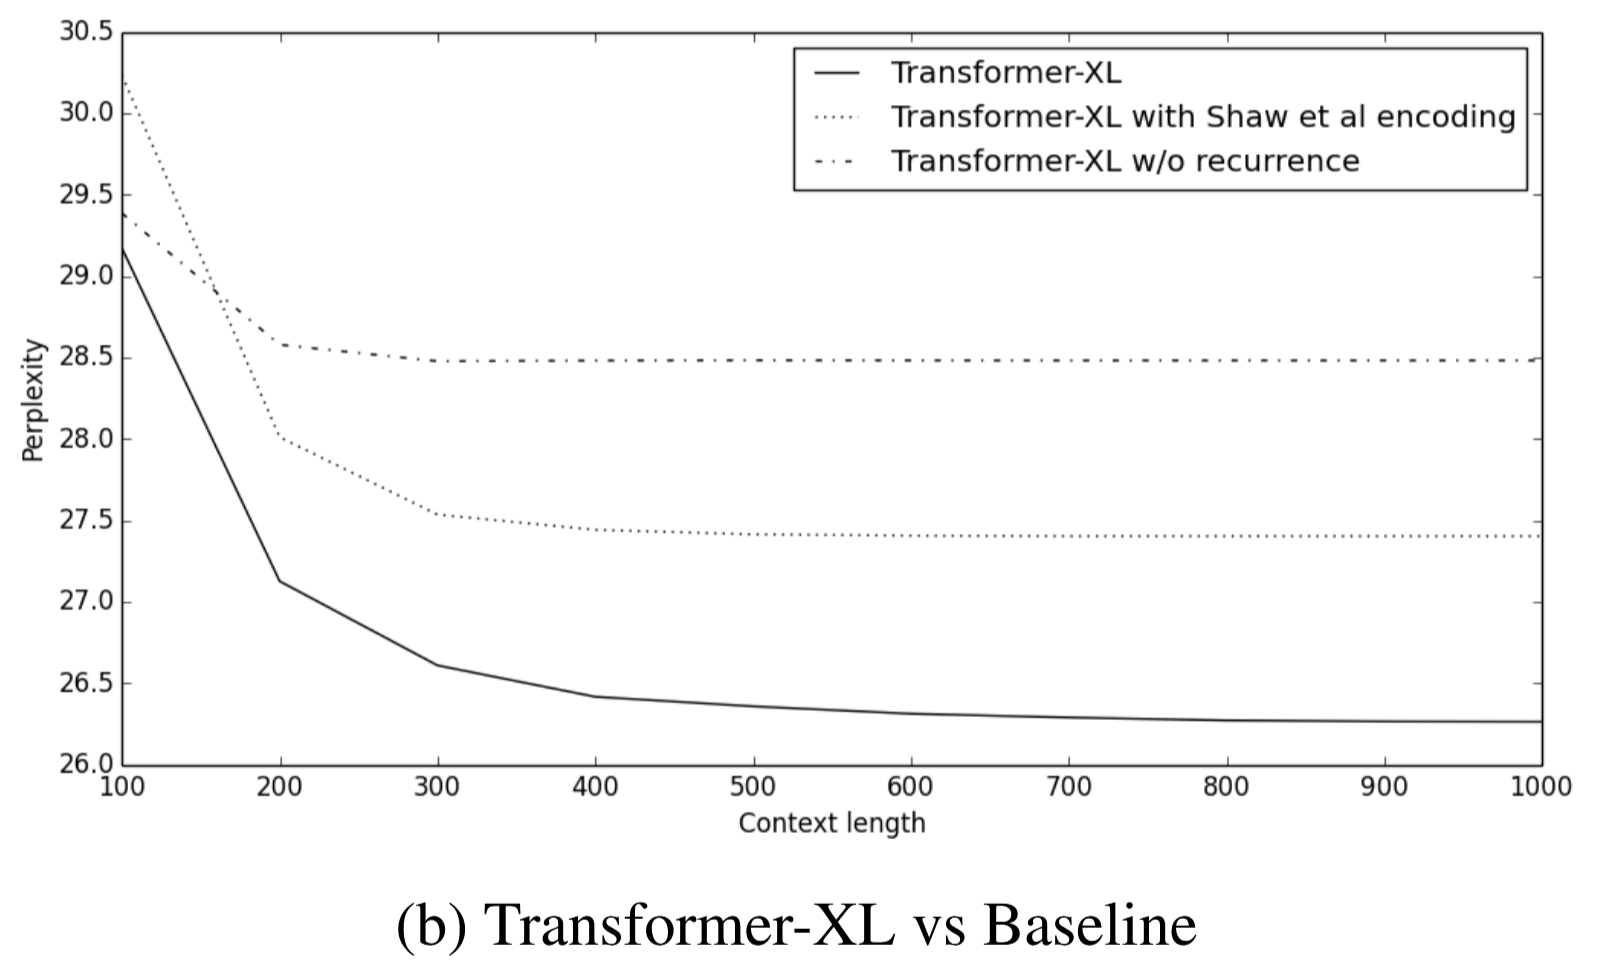
\includegraphics[width=0.5\textwidth]{img/context_length.png}
\caption{Perplexity Score vs. Training Context Length.}
\end{figure}

Furthermore, I want to validate the paper's results that increasing the context window during training results in a "plateau" in the perplexity score, where the model initially sees performance gains, but begins to taper off at a context length of around 400 tokens. This is shown in Figure 1, taken from the paper.

% Since the public GitHub repo provides the code and scripts to download the same datasets used in the paper, I believe getting the same data used by the authors should not be a concern. The main concern I think will be a challenge will be the training phase, since I do not have access to much compute (NVIDIA GTX 3070Ti), and I'm afraid the larger models might not converge quickly enough to acheive the results presented in the paper.

\section{Implementation Status}

The repo provided by the authors was written in Python 2.7 with TensorFlow 1.12.0 (note that these are quite out of date with respect to more modern versions).

\subsection{Pre-Trained Model Evaluation}

The paper provides shell scripts to fetch the pre-trained model checkpoints and data files from their website. The data and checkpoints are in the form of Python .pkl files, so the same Python versions as the authors are required to run the models and reproduce the results. Table 1 shows the results of the pre-trained models compared to what is in the paper.

\begin{center}
\begin{tabular}{ |c|c|c|c| }
 \hline
 Dataset & Metric & Paper & Repro. \\
 \hline
 WikiText-103 & PPL & 18.3 & 18.31 \\ 
 enwiki8 & BPC & 0.99 & 0.936* \\ 
 One Billion Word & PPL & 21.8 & 21.77 \\ 
 text8 & BPC & 1.08 & 1.15** \\
 \hline
\end{tabular}
\begin{tablenotes}
  \item[*] * Run on 300/4828 of total batches of dataset.
  \item[*] ** Run on 26/2442 of total batches of dataset.
  \end{tablenotes}
\end{center}

The paper's results match almost exactly with the model checkpoints provided by the authors. This is quite expected since I necessarily am running the same Python and TensorFlow version with the same models trained by the authors. The only discrepencies are the two datasets that were unable to run to completion (these ran for several hours). Since I am only able to run the original pre-trained models on CPU, that caused a major bottleneck in the inference time. 

The final values for both datasets that did not run to completion are relatively far from the final value, indicating to me there may be contiguous batches of the dataset where the model performs well (likely near the beginning since the reimplementation's result is significantly better than the paper's result), and some batches where it performs worse, likely later in the dataset.

\subsubsection{Technical Challenges}
The major challenge with this part of the expirement is to do with the old tech stack used being incompatible with my system. I am running on Ubuntu 22.04, with an NVIDIA GTX 3070 GPU. The oldest version of CUDA that is supported for my operating system is CUDA 11.7, while the version required for TensorFlow 1.12.0 GPU is 9.0. I tried running the official docker image for TensorFlow 1.12.0 which has CUDA 9.0 pre-installed, but ran into CUDA mismatch related errors. 

Therefore, the only way I could run the model checkpoints and load from the pkl files provided for baseline pre-trained model evaluation would be by running in CPU only, which is significantly slower and is the reason why the entire batch set could not be completed. To do this, I ran the CPU only Tensorflow 1.12.0 docker image instead, which gave me no problems.

\subsection{Model Retraining Pipeline}

Since running with a GPU is effectively required to retrain the models from scratch with any kind of efficiency, it was imperative to upgrade the tech stack used in the paper. To begin, migrating to a newer version of Python and TensorFlow was required to allow my system to utilize the GPU. However, the code was written before TensforFlow 2.0.0 was released, so I needed to follow the TensorFlow 1.0 to 2.0 migration guide (\verb|www.tensorflow.org/guide/migrate|). Once this was done, I needed to run a TensorFlow 2.15.0 Docker container, and I was able to run the updated code. However, due to out of memory issues, the model sizes provided natively were too large to run. For the text8 base model, for example, I had to halve the dimensions of the \verb|D_MODEL|, \verb|D_EMBED|, \verb|TGT_LEN|, and \verb|MEM_LEN| parameters, effectively reducing the model size by a considerable amount so it could fit in memory. This will result in a model that performs worse than the baseline would suggest. At the time of writing this report, the smaller model is still being trained and has a BPC score of 1.9425 in comparison with the 1.08 score mentioned in the paper. I hypothesize that this smaller model may still have a reasonable final score on the training dataset, but may not generalize well to the test dataset.

\subsubsection{Technical Challenges}
The WikiText-103 dataset was not available from the download scripts due to the hosting site being taken down. I was able to find the same files at \hyperlink{https://www.kaggle.com/datasets/rohitgr/wikitext}{this Kaggle website}.

There were several challenges in getting the training scripts to run locally on my machine. I tried upgrading to a very recent TensorFlow version (2.20.0), which relied on Keras 3.0 and was incompatible with my upgraded code. Therefore, I downgraded to TensorFlow 2.15.0 which was compatible with my system and still used the legacy Keras 2.0 model. 

This version worked for running the training scripts, but the model was too large to fit in memory. Halving some model parameters resulted in a model that was able to fit in memory, but had half the parameters (40.9M to 20.5M).

Going forward, I don't think it will be feasible to train these models on my laptop since I only have ~8GB of VRAM in my GPU, so I am more constrained by memory than compute. Therefore, I want to look into using a GPU cluster from my research group to see if I can offload the training onto there. That would hopefully allow me to train the smaller models without needing to downsize them.

\subsection{Varying Context Window Implementation}

This hypothesis will be the most challenging to implement as it involves training multiple models with differing parameters, which is already challenging enough given the size of the models and datasets combined with my machine's limited resources. I think to accomplish this for the final project, I will downsize the model parameters (even if training on a department cluster), since I am more interested in the relative effect that changing the context window size has on the final result compared to the absolute scores.

\section{Future Work and Considerations}
For the final submission, I think the first step going forward will be to find more powerful machines to run the training pipelines on so I am not constrained by memory or compute. I also want to implement frequent model checkpoints since it does not seem the provided training pipeline saves intermediate artifacts during the pipeline, and I have already had it happen multiple times where I would get an error in the middle of training that killed my progress.

Overall, I think my unfamiliarity with TensorFlow as a framework has been challenging since I am having a hard time following the structure of the program. I have enough baseline knowledge to fix bugs as they come up, but I think I require a more fundamental understanding of the framework and the math in the paper to come up with smarter pipeline training decisions. However, most of the findings I've been able to reproduce so far have been consistent with the claims of the paper, and the discrepancies are explainable with the common issue being memory or compute constrained by my hardware.

\section{References}

[1] Z. Dai, Z. Yang, Y. Yang, J. Carbonell, Q. V. Le, and R. Salakhutdinov, “Transformer-XL: Attentive Language Models Beyond a Fixed-Length Context,” arXiv.org, 2019. https://arxiv.org/abs/1901.02860

\end{document}
